\chapter{Evaluation}
\label{sec:evaluation}
\section{Comparison of different models}

\begin{equation}
	F1 = \frac{2 \times \text{TP}}{2 \times \text{TP} + \text{FN} + \text{FP}}
\end{equation}

The F1 score is a statistical measure used to evaluate the precision and recall of a model's predictions, essentially capturing the balance between the model's accuracy and its comprehensiveness in identifying relevant instances. Precision represents the accuracy of positive predictions, while recall measures the model's ability to identify all actual positive instances. The F1 score is the harmonic mean of precision and recall, thus ensuring that both metrics contribute equally to the final score, with a perfect F1 score being 1 and the worst being 0 \cite{chicco-2020}.

\begin{equation}
	\text{Weighted F1} = \sum_{i=1}^{N} w_i \times F1_i
\end{equation}

The weighted F1 score extends this concept by taking into account the class imbalance within a dataset. In scenarios where some classes are more prevalent than others, the weighted F1 score calculates a separate F1 score for each class, giving each score a weight proportional to the number of true instances for each class. This approach prevents the model's performance from being overly influenced by its effectiveness on the more common classes, instead emphasizing its overall performance across all classes. The weighted F1 score is particularly valuable in datasets with significant class imbalances, as it provides a more representative assessment of the model's predictive power \cite{leung-2022}.

\begin{table}[h]
	\centering
	\begin{tabular}{|l|l|l|l|l|}
		\hline
		Model            & weighted-F1 score \\ \hline
		CLIP             & \textbf{0.837}    \\
		Only designation & 0.779             \\
		Benchmark        & 0.814             \\
		\hline
	\end{tabular}
	\caption{Weighted-F1 scores}
	\label{tab:f1scores}
\end{table}

Table \ref{tab:f1scores} displays the range of weighted-F1 scores achieved by our model. These scores were obtained from a test set submitted to the challenge website, for which we did not have direct access to the true labels.

The CLIP model, which uses the designation and description field, as well as the images, got the best performance with an weighted F1 score of 0.837 (on the clean website test set). In contrast, the text-only model, which relies solely on product designations, achieved a weighted F1 score of 0.779 (on the clean website test set). While this model benefits from the informative nature of the product titles, it lacks the additional contex that images provide. The reduction in the weighted F1 score when compared to the full CLIP model underscores the value of incorporating visual features into the classification process.

The benchmark model, established by the challenge organizers, serves as a standard for comparison, achieving a weighted F1 score of 0.814 (on the clean website test set). While this model demonstrates a strong baseline performance, it falls short of the full CLIP model's capabilites.

It can be seen that integrating the images and the text data into one model gives better results than just using the text alone. It highlights the need for models that can effectively synthesize information from multiple sources, providing a more holistic view of the data at hand.

\section{Evaluation based on a confusion matrix}

A confusion matrix is a powerful tool for evaluating the performance of a classification model, providing a visual representation of the model's predictions compared against the actual labels. It not only reveals the instances of correct and incorrect predictions for each class but also uncovers the specific types of errors, such as which classes are being confused with others, enabling a nuanced analysis of the model's strengths and weaknesses \cite{susmaga-2004}.

We split our data into three parts: 80\% for training the model, 10\% for testing it, and another 10\% to validate how well it's doing. The confusion matrix we're looking at is based on this 10\% validation chunk.\\
The model provides an impressive 0.96\% f1 accuracy score on the validation data, we'll see in the future potential reasons why it did not worked as well on the clean website test set.\\

\begin{figure}[H]
	\centering
	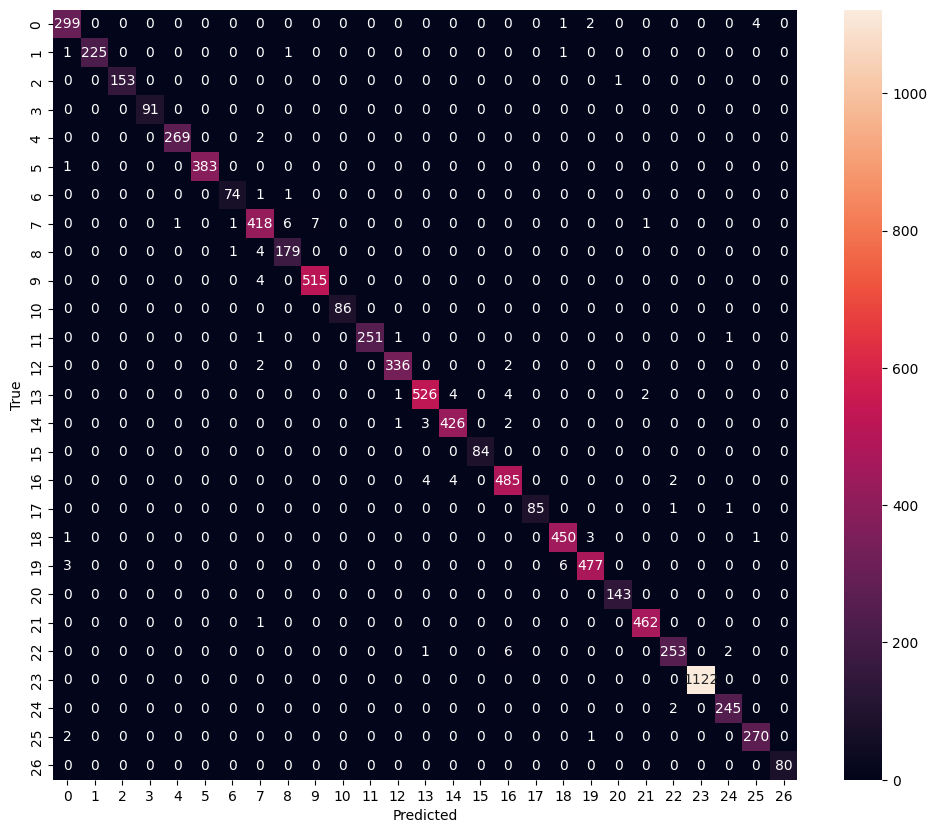
\includegraphics[width=1\textwidth]{confusion_matrix.png}
	\caption{Confusion matrix}
	\label{fig:confusionmatrix}
\end{figure}

The confusion matrix for our model on the evaluation data gives us a clear picture of how well it's guessing the types of products. Most products are being placed in the right categories, which we can tell because there are lots of big numbers forming a diagonal line from the top left to the bottom right. This line shows where the model's guesses match the real answers.

While the model does a great job with many types of products, there are a few areas where it's not as accurate and could be better. But, there aren't too many mistakes overall, which is a good sign that our model isn't just memorizing the training data but actually learning from it.

This is confirmed by how well the model does on a completely new set of products it hasn't seen before (table \ref*{tab:f1scores}: CLIP: 0.837). This means it's pretty good at applying what it's learned to new data.

Even though the confusion matrix might make us think the model has learned the training data too well, its good scores on both the validation data and the new test set from the challenge show that's not the case. It's not just repeating what it saw during training; it's making smart guesses on new products.

From the confusion matrix and the model's scores, it's clear that we've built a strong model that's good at figuring out what category different products belong to. It does well even with products it hasn't seen before, which proves our methods are working well.


\section{Difference between the results on clean test set and our test set}
When training the model, as we said during the previous chapter we took care
to separate the training, valid and test sets, with a ratio of 80\% training, 10%
valid and 10\% test. The test set was not used during the training of the model
and was only used for the final evaluation of the model. The valid set was used
to evaluate the model during the training process. During the training of the
fusion model, we got a weighted F1 score that was really high, with only one
epoch, the F1 score got up to 0.950 and climbed to 0.960 at epoch 7 on the
validation set, so the result was impressive. And we thoughts we would have
comparable results on the website test set.

However, when we tested the model on the website test, the weighted F1
score was only 0.837. This is a big difference between the true value and the
one we got on the training and test data sets. We also note that this is not just
bad luck, because we got exactly the same kind result when we tested a model
that concatenated the results of the feature extraction instead of multiplying
them.

We don’t have an exact answer for this change in behaviour, it looks like
there is some kind of data leakage during our training process, our first idea
was that there were some kind of complete data leakage (train, valid and test
dataset were completely mixed up), however, after careful review of the code we
did not find it but we find some source of potential answer to this phenomenon:

\subsection{Data Leakage Transfer}

When we trained the first text model, we did not paid attention that the train, test and valid dataset were the same as the one we used for the fusion model. So a potential reason for the difference in the results is that the text model contains information of the train, test and valid dataset of the fusion model, so it is easier for the fusion model to predict the result of the test dataset.

\subsection{Vocabulary decision}

As said in \ref{sec:method}, we created a vocabulary by keeping only the words that were present in the product designation of the training dataset (train,valid and test mixed up). Our embedding do not use any kind of pre-training so it should not be a direct reason for the difference in the results, however, we think that it could have an impact on the results. Maybe in the architecture a weakly trained token (a word that appears 0 or 1 time in the dataset) could have a big impact on the results, bigger than the case where the world would not be present (case were the word is not in the vocabulary (clean validation set from the website)). We think that it could be a potential reason for the difference in the results.


\subsection{Difference between the training and testing dataset}

In real world use case, production data (data that will be provided to model inference) can be very different than the collected data for training. So maybe Rakuten added a bit of challenge by providing a test dataset that is  different than the training dataset. We think that it could be a potential reason for the difference in the results. However it is not a very likely because when we tested the previous model (text model with only designation for example) we did not seen that kind of difference.
vided to model inference) can be very different than the collected data for training. So maybe Rakuten added a bit of challenge by providing a test dataset that is  different than the training dataset. We think that it could be a potential reason for the difference in the results. However it is not a very likely because when we tested the previous model (text model with only designation for example) we did not seen that kind of difference.